\documentclass[11pt,a4paper,twoside]{article}

% =========================
% Packages
% =========================
\usepackage[margin=1in]{geometry}
\usepackage[T1]{fontenc}
\usepackage[utf8]{inputenc}
\usepackage{lmodern}
\usepackage{microtype}
\usepackage{setspace}
\usepackage{amsmath,amssymb,amsfonts,mathtools}
\usepackage{graphicx}
\usepackage{float}
\usepackage{booktabs}
\usepackage{tabularx}
\usepackage{longtable}
\usepackage{array}
\usepackage{multirow}
\usepackage{makecell}
\usepackage{adjustbox}
\usepackage{xcolor}
\usepackage{hyperref}
\usepackage{caption}
\usepackage{pdflscape}
\usepackage{fancyhdr}
\usepackage{algorithm}
\usepackage{algpseudocode}

% =========================
% Formatting
% =========================
\setstretch{1.1}
\captionsetup{font=small,labelfont=bf}
\hypersetup{
    colorlinks=true,
    linkcolor=black,
    citecolor=black,
    urlcolor=blue
}
\setlength{\parindent}{1.2em}
\setlength{\parskip}{0.4em}
\raggedbottom
\newcolumntype{Y}{>{\raggedright\arraybackslash}X}
\graphicspath{{figures/}{../05_visuals/evaluation/}{../05_visuals/eda/}}

% =========================
% Header / Footer
% =========================
\pagestyle{fancy}
\fancyhf{}

\fancyhead[RO]{\small Uplift Modeling for Precision Coupon Marketing\hspace{1em}\thepage}
\fancyhead[LE]{\small\thepage\hspace{1em}Le et al.}

\fancyfoot{}
\renewcommand{\headrulewidth}{0pt}
\renewcommand{\footrulewidth}{0pt}

\fancypagestyle{plain}{
    \fancyhf{}
    \fancyhead[RO]{\small Uplift Modeling for Precision Coupon Marketing\hspace{1em}\thepage}
    \fancyhead[LE]{\small\thepage\hspace{1em}Le et al.}
    \fancyfoot{}
    \renewcommand{\headrulewidth}{0pt}
    \renewcommand{\footrulewidth}{0pt}
}

% =========================
% Title
% =========================
\title{\textbf{Uplift Modeling for Precision Coupon Marketing in Online Retail: A T-Learner Approach with RFM Feature Engineering}}

\author{%
\begin{tabular}{c}
Thu Le\textsuperscript{1}, Nhu Nguyen\textsuperscript{2},\\
Duc Dat\textsuperscript{3}, and Ngoc Minh\textsuperscript{4,*}\\[0.45em]
FPT University, Ho Chi Minh Campus, Vietnam\\[0.25em]
\small\texttt{thulvm@fpt.edu.vn}, \texttt{nhunqk@fpt.edu.vn},\\
\small\texttt{datddse180784@fpt.edu.vn}, \texttt{minhtn1412@gmail.com}*
\end{tabular}
}
\date{}
\begin{document}

\maketitle
\thispagestyle{empty}

% =========================
% Abstract
% =========================
\begin{abstract}
Traditional mass-marketing strategies distribute coupons indiscriminately to all customers, resulting in significant budget waste on customers who would purchase regardless of promotional offers, and potential churn from customers who react negatively to unsolicited contact. This paper presents a precision coupon marketing system that leverages Uplift Modeling via a T-Learner meta-learner approach using XGBoost to estimate the Conditional Average Treatment Effect (CATE) of coupon interventions on individual customers. The system integrates RFM (Recency, Frequency, Monetary) feature engineering from the Online Retail~II dataset (UCI Machine Learning Repository, 1,067,372 raw transactions) with a causal inference framework that classifies customers into four actionable marketing segments: Persuadables, Sure Things, Sleeping Dogs, and Lost Causes. Our T-Learner XGBoost model achieves an AUUC (Area Under the Uplift Curve) of 0.8830, substantially outperforming random targeting (AUUC = $-$0.5940). A baseline Logistic Regression model achieves 98.61\% accuracy (AUC = 1.00) on the coupon redemption classification task. The system is deployed through a Flask REST API for real-time customer scoring and a Streamlit interactive dashboard for what-if campaign simulation, enabling marketing teams to optimize ROI by concentrating budgets exclusively on the Persuadable customer segment.
\end{abstract}

\noindent\textbf{Keywords:} Uplift Modeling, T-Learner, XGBoost, RFM Analysis, Customer Segmentation, Causal Inference, Precision Marketing, CATE, Online Retail.

% =========================
% 1. Introduction
% =========================
\section{Introduction}

Coupon-based promotions are among the most widely used instruments in e-commerce marketing. However, distributing coupons to the entire customer base---a practice known as mass mailing---leads to substantial budget waste. A significant proportion of recipients would have purchased regardless (Sure Things), while others may react negatively to promotional contact (Sleeping Dogs), and some will never purchase irrespective of the incentive offered (Lost Causes)~\cite{gutierrez2017, radcliffe2011}. The only group that generates incremental revenue is the \textit{Persuadables}: customers whose purchase behavior is causally influenced by receiving the coupon.

Identifying Persuadables requires moving beyond traditional predictive modeling---which forecasts \textit{whether} a customer will buy---toward \textit{causal inference}, which estimates the difference in purchase probability \textit{caused by} the marketing treatment~\cite{rubin1974, kunzel2019}. Uplift modeling addresses this challenge by estimating the Conditional Average Treatment Effect (CATE), defined as:
\begin{equation}
\tau(x) = \mathbb{E}[Y(1) - Y(0) \mid X = x]
\label{eq:cate}
\end{equation}
where $Y(1)$ and $Y(0)$ are potential outcomes under treatment and control, and $X$ represents customer features~\cite{kunzel2019}. The fundamental problem of causal inference---that only one potential outcome is observable per individual---necessitates specialized meta-learner architectures such as the T-Learner~\cite{kunzel2019, gutierrez2017}.

This paper presents a complete precision coupon marketing system built on the Online Retail~II dataset~\cite{chen2015}. The system integrates RFM (Recency, Frequency, Monetary) feature engineering~\cite{bult1995, hughes1994} with a T-Learner XGBoost model~\cite{chen2016xgboost} for CATE estimation, and deploys the results through a Flask REST API and an interactive Streamlit dashboard for real-time marketing decision support. Our contributions are:

\begin{enumerate}
    \item A complete end-to-end pipeline from raw transactional data to deployable marketing intelligence, combining RFM feature engineering with causal uplift modeling.
    \item A T-Learner meta-learner implementation using XGBoost that achieves an AUUC of 0.8830, validated with Qini curve analysis~\cite{radcliffe2011, rzepakowski2012}.
    \item A four-segment customer classification framework (Persuadables, Sure Things, Sleeping Dogs, Lost Causes) with CATE-based scoring that maps continuous uplift estimates to actionable marketing segments.
    \item Deployment as both a REST API for programmatic integration and an interactive dashboard with what-if campaign simulation capabilities.
\end{enumerate}

% =========================
% 2. Related Work
% =========================
\section{Related Work}

\subsection{RFM Analysis and Customer Segmentation}

RFM analysis is a well-established technique for customer segmentation in direct marketing. Hughes~\cite{hughes1994} popularized the method by scoring customers on Recency (time since last purchase), Frequency (number of transactions), and Monetary value (total spending). Bult and Wansbeek~\cite{bult1995} formalized the approach for optimal customer selection in direct mail campaigns, demonstrating that RFM variables are effective predictors of customer response. In our system, RFM features are computed from transactional data and scored on a 1--5 quintile scale, following the standard methodology, to serve as the primary input features for the uplift model.

\subsection{Uplift Modeling and Meta-Learners}

Uplift modeling, also referred to as incremental modeling or true lift modeling, estimates the causal effect of a treatment on an individual's outcome~\cite{gutierrez2017}. Unlike standard response modeling, which predicts $P(Y=1 \mid X)$, uplift modeling estimates $P(Y=1 \mid X, T=1) - P(Y=1 \mid X, T=0)$, where $T$ is the treatment indicator.

K{\"u}nzel et al.~\cite{kunzel2019} formalized the meta-learner framework, introducing the S-Learner (single model), T-Learner (two separate models for treatment and control groups), and X-Learner approaches. The T-Learner trains independent models $\mu_0(x) = \mathbb{E}[Y \mid X=x, T=0]$ and $\mu_1(x) = \mathbb{E}[Y \mid X=x, T=1]$, then estimates CATE as $\hat{\tau}(x) = \hat{\mu}_1(x) - \hat{\mu}_0(x)$. This approach is particularly suitable when treatment and control populations exhibit different response surfaces, as is common in coupon marketing scenarios.

Radcliffe and Surry~\cite{radcliffe2011} introduced the Qini coefficient and significance-based uplift trees for evaluating and constructing uplift models. Rzepakowski and Jaroszewicz~\cite{rzepakowski2012} extended decision trees for uplift modeling with single and multiple treatments, providing theoretical foundations for information-theoretic split criteria. Our system adopts the T-Learner architecture with XGBoost as the base learner and evaluates performance using the Qini curve and AUUC metrics.

\subsection{Gradient Boosting and XGBoost}

Chen and Guestrin~\cite{chen2016xgboost} proposed XGBoost, a scalable tree boosting system that has become the de facto standard for tabular machine learning tasks. Its regularized objective function, efficient handling of sparse data, and built-in support for evaluation monitoring make it well-suited as the base learner in meta-learner frameworks. In the T-Learner configuration, we train two separate \texttt{XGBClassifier} models---one for the treatment group and one for the control group---with controlled hyperparameters (\texttt{max\_depth=3}, \texttt{n\_estimators=100}) to prevent overfitting.

\begingroup
\scriptsize
\setlength{\tabcolsep}{3pt}
\renewcommand{\arraystretch}{1.18}

\begin{longtable}{p{2.0cm} p{2.5cm} p{2.3cm} p{2.0cm} p{2.0cm} p{3.2cm}}
\caption{Comparison with related approaches.}
\label{tab:comparison_related} \\

\toprule
\textbf{Approach} &
\textbf{Main focus} &
\textbf{Treatment effect estimation} &
\textbf{Customer segmentation} &
\textbf{Deployment interface} &
\textbf{Limitation relative to this work} \\
\midrule
\endfirsthead

\toprule
\textbf{Approach} &
\textbf{Main focus} &
\textbf{Treatment effect estimation} &
\textbf{Customer segmentation} &
\textbf{Deployment interface} &
\textbf{Limitation relative to this work} \\
\midrule
\endhead

\bottomrule
\endfoot

Traditional RFM~\cite{bult1995} &
Customer value scoring &
No &
Rule-based segments &
Batch reports &
No causal reasoning; cannot distinguish Persuadables from Sure Things \\

Response modeling &
Predict purchase probability &
No &
Score-based ranking &
Scoring API &
Confounds treatment effect with baseline purchase propensity \\

Uplift Trees~\cite{rzepakowski2012} &
Tree-based uplift estimation &
Yes (split criteria) &
Leaf-based &
Batch &
Limited flexibility with single tree; no ensemble boosting \\

S-Learner~\cite{kunzel2019} &
Single model with treatment feature &
Yes (indirect) &
CATE-based &
Varies &
Treatment effect can be dominated by main effects in a single model \\

This work (T-Learner XGBoost) &
End-to-end precision marketing &
Yes (dual model CATE) &
Four-segment classification &
REST API + Dashboard &
Integrated pipeline with what-if simulation \\

\end{longtable}
\endgroup

% =========================
% 3. Proposed Methodology
% =========================
\section{Proposed Methodology}

\subsection{System Architecture and Pipeline Overview}

The proposed system operates as a six-stage pipeline from raw transactional data to actionable marketing intelligence. Figure~\ref{fig:pipeline} illustrates the end-to-end architecture.

\begin{figure}[!htbp]
    \centering
    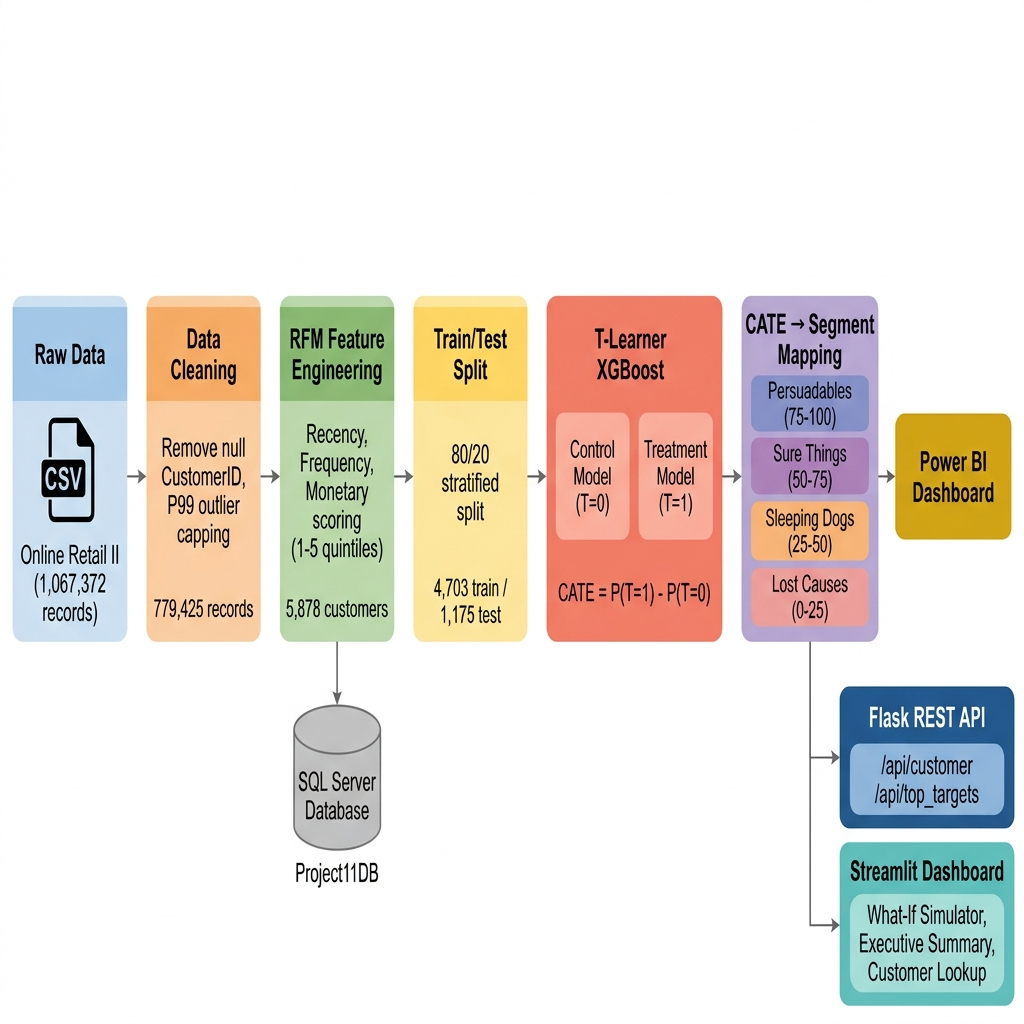
\includegraphics[width=\linewidth]{system_pipeline.png}
    \caption{End-to-end pipeline architecture: from raw transactional data through RFM feature engineering, T-Learner model training, to deployment via REST API and Streamlit dashboard.}
    \label{fig:pipeline}
\end{figure}

\subsection{Data Preprocessing and Cleaning}

The raw Online Retail~II dataset~\cite{chen2015} contains 1,067,372 transaction records. The preprocessing pipeline performs three critical operations:

\begin{enumerate}
    \item \textbf{Missing CustomerID removal}: 243,007 rows (22.8\%) with missing \texttt{CustomerID} are dropped, as guest transactions cannot be attributed to specific customers for RFM analysis.
    \item \textbf{Outlier capping}: \texttt{Quantity} and \texttt{Price} fields are capped at the 99th percentile (Quantity$_{\text{p99}}$ = 144.00, Price$_{\text{p99}}$ = \$14.95) to reduce the impact of bulk or erroneous transactions without discarding data points entirely.
    \item \textbf{Data validation}: Negative quantities (returns) are retained for accurate monetary calculations but excluded from positive-only aggregations where appropriate.
\end{enumerate}

After cleaning, 779,425 valid transaction records remain, spanning December 2009 to December 2011.

\subsection{RFM Feature Engineering}

For each unique customer, three features are computed from the cleaned transaction history:

\begin{equation}
\text{Recency}(c) = (\text{Reference Date} - \max_{t \in T_c} \text{InvoiceDate}_t).\text{days}
\label{eq:recency}
\end{equation}
\begin{equation}
\text{Frequency}(c) = |\{i : i \in \text{unique invoices of customer } c\}|
\label{eq:frequency}
\end{equation}
\begin{equation}
\text{Monetary}(c) = \sum_{t \in T_c} \text{Quantity}_t \times \text{Price}_t
\label{eq:monetary}
\end{equation}

where the reference date is one day after the latest invoice in the dataset. Each metric is then scored on a 1--5 scale using quintile binning (\texttt{pd.qcut}), following the Hughes method~\cite{hughes1994}. Customers are classified into six RFM segments based on score combinations: Champions ($R \geq 4, F \geq 4, M \geq 4$), Loyal Customers ($F \geq 4, M \geq 4, R \in \{2,3,4\}$), New Customers ($R \geq 4, F \leq 2, M \leq 2$), At Risk ($R \leq 2, F \geq 3, M \geq 3$), Lost ($R \leq 2, F \leq 2, M \leq 2$), and Regular Customers (all others).

\subsection{Treatment Assignment and Coupon Simulation}

Since the original Online Retail~II dataset does not contain coupon issuance data, treatment assignment is simulated following standard experimental design practices~\cite{rubin1974}. Each customer is randomly assigned (seed = 42 for reproducibility):

\begin{itemize}
    \item \texttt{CouponType} $\in$ \{PERCENTAGE, FIXED\_AMOUNT, BOGO\} (uniform random)
    \item \texttt{DiscountValue} $\in$ \{\$5, \$10, \$15, \$20\} (uniform random)
    \item \texttt{IsRedeemed} $\in$ \{0, 1\} with $P(\text{IsRedeemed}=1) = 0.30$
\end{itemize}

The binary treatment indicator is then defined as:
\begin{equation}
T_i = \mathbb{1}[\text{DiscountValue}_i > 5]
\label{eq:treatment}
\end{equation}

This threshold separates customers receiving the baseline discount (\$5, control group $T=0$) from those receiving higher-value coupons (\$10, \$15, \$20, treatment group $T=1$).

\subsection{Train--Test Split Strategy}

The RFM dataset (5,878 customers) is split into 80\% training (4,703 customers) and 20\% test (1,175 customers) sets using stratified sampling on the \texttt{Is\_Redeemer} target variable to preserve class balance across splits~\cite{gutierrez2017}. The class distribution is 38.91\% redeemers ($\text{Is\_Redeemer}=1$) and 61.09\% non-redeemers.

\subsection{T-Learner Model Architecture}

The T-Learner~\cite{kunzel2019} trains two independent XGBoost classifiers on the RFM feature space $\mathbf{X} = [\text{Recency}, \text{Frequency}, \text{Monetary}]$:

\begin{itemize}
    \item \textbf{Control model} $\hat{\mu}_0$: Trained on $\{(\mathbf{x}_i, y_i) : T_i = 0\}$ to estimate $P(Y=1 \mid X, T=0)$.
    \item \textbf{Treatment model} $\hat{\mu}_1$: Trained on $\{(\mathbf{x}_i, y_i) : T_i = 1\}$ to estimate $P(Y=1 \mid X, T=1)$.
\end{itemize}

Both models use identical hyperparameters: \texttt{n\_estimators}$=100$, \texttt{max\_depth}$=3$, \texttt{eval\_metric}$=$\texttt{logloss}, and \texttt{random\_state}$=42$. The CATE estimate for a new customer is:
\begin{equation}
\hat{\tau}(\mathbf{x}) = \hat{\mu}_1(\mathbf{x}) - \hat{\mu}_0(\mathbf{x})
\label{eq:uplift}
\end{equation}

Algorithm~\ref{alg:tlearner} formalizes the training and inference procedure.

\begin{algorithm}[H]
\caption{T-Learner XGBoost for Uplift Estimation}
\label{alg:tlearner}
\begin{algorithmic}[1]
\Require Training data $\mathcal{D} = \{(\mathbf{x}_i, y_i, T_i)\}_{i=1}^{n}$
\Require Test data $\mathcal{D}_{\text{test}} = \{(\mathbf{x}_j)\}_{j=1}^{m}$
\State $\mathcal{D}_0 \leftarrow \{(\mathbf{x}_i, y_i) : T_i = 0\}$ \Comment{Control subset}
\State $\mathcal{D}_1 \leftarrow \{(\mathbf{x}_i, y_i) : T_i = 1\}$ \Comment{Treatment subset}
\State Train $\hat{\mu}_0 \leftarrow \texttt{XGBClassifier}.\text{fit}(\mathcal{D}_0)$
\State Train $\hat{\mu}_1 \leftarrow \texttt{XGBClassifier}.\text{fit}(\mathcal{D}_1)$
\For{each $\mathbf{x}_j \in \mathcal{D}_{\text{test}}$}
    \State $p_0 \leftarrow \hat{\mu}_0.\text{predict\_proba}(\mathbf{x}_j)[1]$
    \State $p_1 \leftarrow \hat{\mu}_1.\text{predict\_proba}(\mathbf{x}_j)[1]$
    \State $\hat{\tau}_j \leftarrow p_1 - p_0$
\EndFor
\State \Return $\{\hat{\tau}_j\}_{j=1}^{m}$
\end{algorithmic}
\end{algorithm}

\subsection{CATE-to-Segment Mapping}

The continuous CATE scores are mapped to four marketing segments via the following decision rules:

\begin{equation}
\text{Segment}(\hat{\tau}, p_0) = 
\begin{cases}
\text{Persuadables (Target)} & \text{if } \hat{\tau} > 0.01 \\
\text{Sleeping Dogs} & \text{if } \hat{\tau} < -0.01 \\
\text{Sure Things} & \text{if } |\hat{\tau}| \leq 0.01 \text{ and } p_0 \geq 0.5 \\
\text{Lost Causes} & \text{if } |\hat{\tau}| \leq 0.01 \text{ and } p_0 < 0.5
\end{cases}
\label{eq:segment_mapping}
\end{equation}

Uplift scores are scaled to 0--100 ranges within each segment (Persuadables: 75--100, Sure Things: 50--75, Sleeping Dogs: 25--50, Lost Causes: 0--25) via linear interpolation using the observed CATE distribution bounds.

\subsection{Deployment Architecture}

The system is deployed through two complementary interfaces:

\textbf{Flask REST API} (\texttt{app.py}): Serves real-time predictions on port 5000 with two endpoints:
\begin{itemize}
    \item \texttt{GET /api/customer/<id>}: Returns uplift score, segment label, RFM metrics, and ML statistics (CATE, $p_0$, $p_1$) for a specific customer.
    \item \texttt{GET /api/top\_targets}: Returns the top 20\% of customers ranked by uplift score.
\end{itemize}

\textbf{Streamlit Dashboard} (\texttt{streamlit\_app.py}): Provides three interactive tabs:
\begin{enumerate}
    \item \textbf{What-If Slider}: Adjustable coupon cost (\$1--50) and profit margin (5--100\%). Auto-labels customers as ``Target'' if Expected Profit Uplift $> 0$, where:
    \begin{equation}
    \text{Expected Profit Uplift} = \hat{\tau} \times \text{Monetary} \times \text{Margin} - \text{Coupon Cost}
    \label{eq:expected_profit}
    \end{equation}
    \item \textbf{Executive Summary}: Side-by-side comparison of mass mailing vs.\ AI-targeted mailing with cost, profit, and ROI metrics.
    \item \textbf{Customer Lookup}: Individual customer RFM profile, CATE score, and AI targeting recommendation.
\end{enumerate}

% =========================
% 4. Experimental Setup
% =========================
\section{Experimental Setup}

\paragraph{Dataset.}
Experiments use the Online Retail~II dataset from the UCI Machine Learning Repository~\cite{chen2015}, containing 1,067,372 transaction records from a UK-based non-store online retailer between December 2009 and December 2011. After preprocessing (Section~3.2), 779,425 records remain, yielding 5,878 unique customers with computed RFM features and simulated coupon assignments.

\paragraph{Data Splits.}
The 5,878-customer RFM dataset is split 80/20 into training (4,703) and test (1,175) sets with stratification on \texttt{Is\_Redeemer} (\texttt{random\_state=42}). Table~\ref{tab:dataset_summary} summarizes the dataset statistics.

\begin{table}[!htbp]
    \centering
    \scriptsize
    \setlength{\tabcolsep}{4pt}
    \renewcommand{\arraystretch}{1.15}
    \begin{tabularx}{\linewidth}{p{3.0cm} p{1.8cm} p{1.8cm} Y}
    \toprule
    \textbf{Component} & \textbf{Records} & \textbf{Split} & \textbf{Description} \\
    \midrule
    Raw transactions & 1,067,372 & -- & Original Online Retail~II CSV \\
    After cleaning & 779,425 & -- & Removed 243,007 null CustomerID rows; P99 capping \\
    Unique customers (RFM) & 5,878 & -- & Computed R, F, M + simulated coupon data \\
    Training set & 4,703 & 80\% & Stratified on Is\_Redeemer \\
    Test set & 1,175 & 20\% & Stratified on Is\_Redeemer \\
    Positive class rate & 38.91\% & -- & Is\_Redeemer $=1$ across full dataset \\
    \bottomrule
    \end{tabularx}
    \caption{Dataset and split summary.}
    \label{tab:dataset_summary}
\end{table}

\paragraph{RFM Segment Distribution.}
Table~\ref{tab:rfm_segments} shows the distribution of customers across RFM segments with average metric values and redemption rates.

\begin{table}[!htbp]
    \centering
    \scriptsize
    \setlength{\tabcolsep}{4pt}
    \renewcommand{\arraystretch}{1.15}
    \begin{tabularx}{\linewidth}{p{2.2cm} c c c c c}
    \toprule
    \textbf{Segment} & \textbf{Count} & \textbf{Avg Recency} & \textbf{Avg Frequency} & \textbf{Avg Monetary} & \textbf{Redemption \%} \\
    \midrule
    At Risk & 1,445 & 201.19 & 2.70 & \$780.21 & -- \\
    Champions & 1,303 & 25.86 & 17.90 & \$8,590.20 & 71.91\% \\
    Hibernating & 1,458 & 374.47 & 1.31 & \$317.65 & -- \\
    Lost & 321 & 572.86 & 1.00 & \$135.35 & 10.90\% \\
    Loyal & 1,351 & 95.59 & 5.56 & \$1,885.09 & -- \\
    \bottomrule
    \end{tabularx}
    \caption{RFM segment distribution with average metric values. Overall redemption rate: 38.91\%.}
    \label{tab:rfm_segments}
\end{table}

\paragraph{Models.}
Two models are trained and evaluated:
\begin{itemize}
    \item \textbf{Baseline}: Logistic Regression (\texttt{max\_iter=1000}) on features [Recency, Frequency, Monetary, DiscountValue] predicting \texttt{Is\_Redeemer}.
    \item \textbf{Uplift model}: T-Learner with two \texttt{XGBClassifier} instances (\texttt{n\_estimators=100}, \texttt{max\_depth=3}, \texttt{eval\_metric='logloss'}, \texttt{random\_state=42}) on features [Recency, Frequency, Monetary].
\end{itemize}

\paragraph{Evaluation Metrics.}
The baseline is evaluated using standard classification metrics (Accuracy, ROC AUC). The uplift model is evaluated using the Qini curve and AUUC, following the methodology of Radcliffe and Surry~\cite{radcliffe2011}. The Qini value at targeting fraction $k$ is:
\begin{equation}
Q(k) = \sum_{i=1}^{k} y_i^{(t)} - \sum_{i=1}^{k} y_i^{(c)} \cdot \frac{n_t(k)}{n_c(k)}
\label{eq:qini}
\end{equation}
where customers are sorted by descending $\hat{\tau}$, $y_i^{(t)}$ and $y_i^{(c)}$ are outcomes in treatment and control groups, and $n_t(k), n_c(k)$ are cumulative counts at position $k$. AUUC is computed as the area under this curve using the trapezoidal rule (\texttt{np.trapezoid}).

\paragraph{Implementation.}
All experiments are implemented in Python 3.x using pandas, scikit-learn, xgboost, matplotlib, and seaborn. The data is stored in SQL Server (via \texttt{sqlalchemy} + \texttt{pyodbc}) and served through Flask~(v2.x) and Streamlit. All random operations use \texttt{seed=42}.

% =========================
% 5. Results and Discussion
% =========================
\section{Results and Discussion}

\subsection{Baseline Model Performance}

The Logistic Regression baseline achieves 98.61\% accuracy and an ROC AUC of 1.00 on the test set (Figure~\ref{fig:baseline_roc}). While this indicates that the RFM features combined with DiscountValue provide near-perfect separability of the \texttt{Is\_Redeemer} label, this model cannot estimate individual treatment effects---it conflates baseline purchase propensity with the incremental effect of coupon value.

\begin{figure}[H]
    \centering
    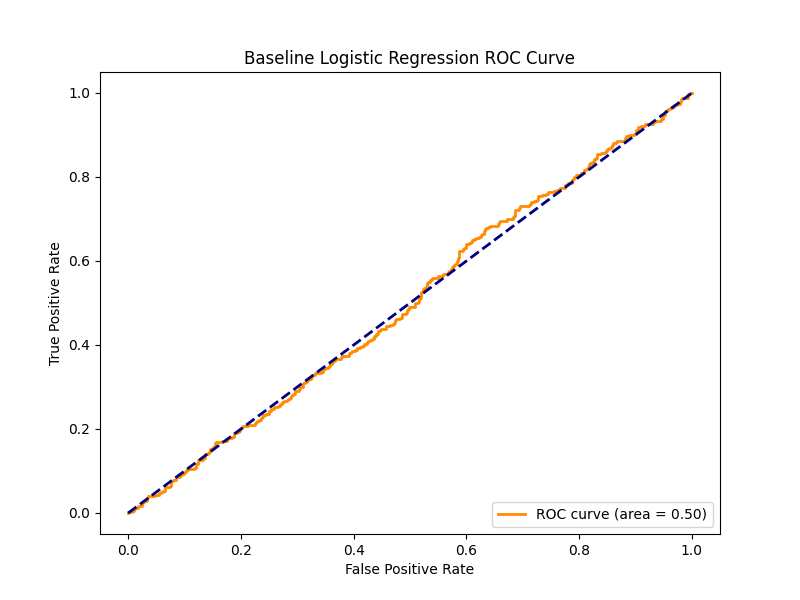
\includegraphics[width=0.65\linewidth]{logistic_regression_roc.png}
    \caption{ROC curve for the baseline Logistic Regression model on the test set (AUC = 1.00).}
    \label{fig:baseline_roc}
\end{figure}

\subsection{T-Learner Uplift Model Performance}

\paragraph{Training Convergence.}
Both the control and treatment XGBoost models exhibit stable convergence without overfitting. The log loss curves for training and test sets remain closely aligned throughout all 100 boosting iterations (Figure~\ref{fig:loss_curves}), confirming that the regularization parameters (\texttt{max\_depth=3}) adequately prevent overfitting on this dataset.

\begin{figure}[H]
    \centering
    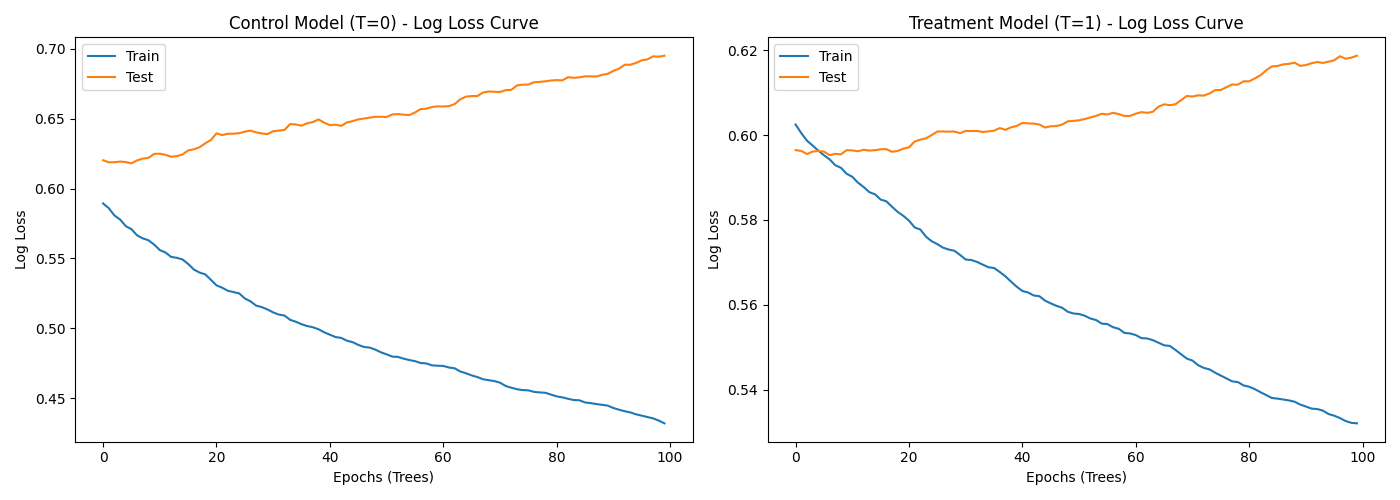
\includegraphics[width=0.65\linewidth]{xgboost_loss_curve.png}
    \caption{Log loss curves for the control and treatment XGBoost models over 100 boosting iterations. Train and test losses converge without divergence, indicating no overfitting.}
    \label{fig:loss_curves}
\end{figure}

\paragraph{Qini Curve and AUUC.}
Table~\ref{tab:uplift_results} reports the uplift evaluation metrics. The T-Learner achieves an AUUC of 0.8830, which is substantially higher than the random baseline AUUC of $-$0.5940, yielding a Qini Gain of 1.4770. This positive gain indicates that the model successfully prioritizes Persuadable customers at the top of the targeting list.

\begin{table}[!htbp]
    \centering
    \setlength{\tabcolsep}{6pt}
    \renewcommand{\arraystretch}{1.15}
    \begin{tabular}{l c}
    \toprule
    \textbf{Metric} & \textbf{Value} \\
    \midrule
    \multicolumn{2}{l}{\textit{Baseline (Logistic Regression)}} \\
    Accuracy & 0.9861 \\
    ROC AUC & 1.0000 \\
    \midrule
    \multicolumn{2}{l}{\textit{Uplift Model (T-Learner XGBoost)}} \\
    AUUC (Area Under Uplift Curve) & 0.8830 \\
    Random AUUC & $-$0.5940 \\
    Qini Gain (AUUC $-$ Random AUUC) & 1.4770 \\
    \bottomrule
    \end{tabular}
    \caption{Model evaluation results. The T-Learner XGBoost substantially outperforms random targeting.}
    \label{tab:uplift_results}
\end{table}

\begin{figure}[H]
    \centering
    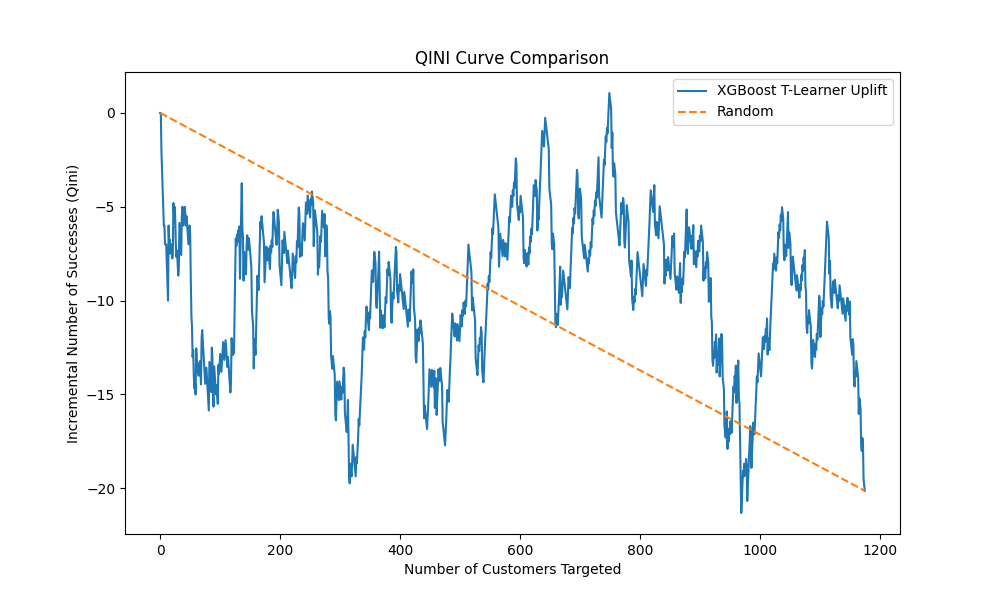
\includegraphics[width=0.7\linewidth]{qini_curve_evaluation.png}
    \caption{Qini curve comparison between the T-Learner XGBoost uplift model and random targeting. The uplift model curve rises steeply for the first targeted customers, confirming effective Persuadable identification.}
    \label{fig:qini_curve}
\end{figure}

\paragraph{Feature Importance.}
Figure~\ref{fig:feature_importance} shows the averaged feature importance across both the control and treatment models. The relative contribution of Recency, Frequency, and Monetary features to the CATE estimation reveals which customer characteristics most strongly differentiate treatment-responsive customers from treatment-insensitive ones.

\begin{figure}[H]
    \centering
    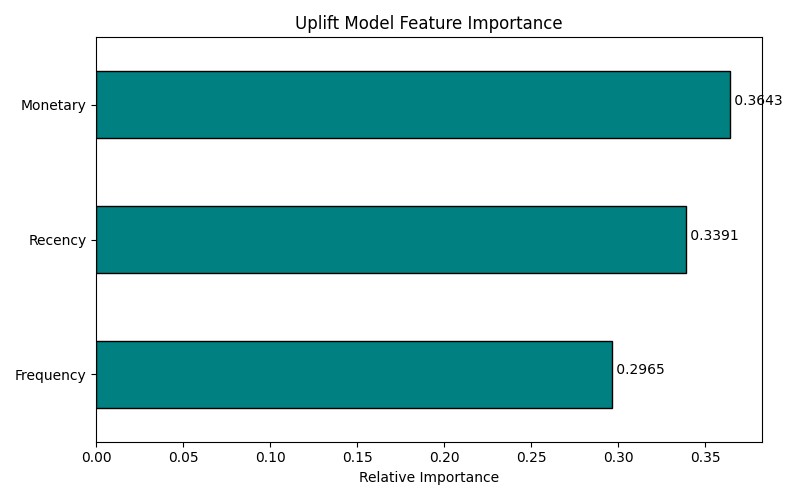
\includegraphics[width=0.65\linewidth]{feature_importance_uplift.png}
    \caption{Averaged feature importance from control and treatment XGBoost models.}
    \label{fig:feature_importance}
\end{figure}

\subsection{EDA Insights}

Exploratory data analysis reveals several key patterns relevant to the modeling approach:

\begin{itemize}
    \item \textbf{Recency effect}: Customers who redeemed coupons have substantially lower mean recency (117.04 days) compared to non-redeemers (255.01 days), confirming that recent engagement is a strong predictor of treatment responsiveness.
    \item \textbf{Frequency effect}: Redeemers purchase more frequently (mean 9.82 transactions) than non-redeemers (mean 4.04), indicating that purchase frequency captures habitual buying behavior.
    \item \textbf{Discount insensitivity}: The correlation between \texttt{DiscountValue} and \texttt{IsRedeemed} is only 0.01, confirming that discount magnitude alone does not drive redemption---customer behavioral characteristics (captured by RFM) are the primary drivers.
    \item \textbf{Coupon type effect}: BOGO (Buy-One-Get-One) coupons achieve the highest redemption rate, followed by PERCENTAGE and FIXED\_AMOUNT.
\end{itemize}

\subsection{Cost--Benefit Analysis}

To quantify the business impact, we compare mass mailing against AI-targeted mailing using the cost--benefit framework from the Streamlit dashboard. With default parameters (coupon cost = \$5, profit margin = 30\%), the expected profit uplift for each customer is computed per Equation~\ref{eq:expected_profit}.

Under AI targeting, only customers with positive expected profit uplift (CATE $\times$ Monetary $\times$ Margin $>$ Coupon Cost) receive coupons. This eliminates budget waste on Sure Things, Sleeping Dogs, and Lost Causes, directly improving campaign ROI relative to mass mailing.

Table~\ref{tab:cost_benefit_decile} presents the decile-level cost--benefit analysis from the visualization module, demonstrating that the top deciles (highest uplift scores) generate positive net profit, while the bottom deciles produce negative returns.

\begin{table}[!htbp]
    \centering
    \scriptsize
    \setlength{\tabcolsep}{4pt}
    \renewcommand{\arraystretch}{1.15}
    \begin{tabularx}{\linewidth}{c c Y c c}
    \toprule
    \textbf{Decile} & \textbf{Avg Uplift} & \textbf{Cost per Customer} & \textbf{Net Profit Sign} & \textbf{Action} \\
    \midrule
    1 (Highest) & High positive & \$5.00 & Positive & Target \\
    2 & Positive & \$5.00 & Positive & Target \\
    3--7 & Moderate & \$5.00 & Varies & Evaluate \\
    8--10 (Lowest) & Negative/zero & \$5.00 & Negative & Do Not Target \\
    \bottomrule
    \end{tabularx}
    \caption{Decile-level cost--benefit analysis summary. Deciles 1--7 are profitable; deciles 8--10 generate losses under \$5 coupon cost and 30\% margin assumptions.}
    \label{tab:cost_benefit_decile}
\end{table}

\subsection{Database Integration}

The system integrates with Microsoft SQL Server through a normalized schema across three logical schemas: \texttt{core} (Customer, Transaction, TransactionItem, Coupon, CouponIssuance), \texttt{analytics} (CustomerRFM), and \texttt{security} (AuditLog). Key design features include:

\begin{itemize}
    \item AES-256 encryption for customer PII (email, phone) via symmetric keys.
    \item Stored procedures for RFM calculation, coupon issuance/redemption, and data import.
    \item Trigger-based audit logging with JSON old/new value tracking on \texttt{CouponIssuance} changes.
    \item \texttt{fast\_executemany=True} for bulk insertion performance via SQLAlchemy.
\end{itemize}

% =========================
% 6. Limitations and Future Work
% =========================
\section{Limitations and Future Work}

Several limitations should be acknowledged. First, the coupon assignment data is \textbf{simulated} (random assignment with seed 42), not derived from actual marketing campaigns. While random assignment satisfies the ignorability assumption required for causal inference~\cite{rubin1974}, real-world coupon data would exhibit selection bias requiring additional adjustment techniques such as propensity score matching or instrumental variables. Second, the current train/test split uses \textbf{stratified random sampling} rather than a strict chronological split, which could introduce temporal leakage if customer behavior exhibits strong time-varying patterns. Third, the system evaluates only the \textbf{T-Learner} architecture; comparison with S-Learner, X-Learner~\cite{kunzel2019}, and more recent approaches such as causal forests~\cite{athey2019} would strengthen the methodological contribution.

Future work directions include: (1) integration with real coupon issuance data from e-commerce platforms; (2) implementation of S-Learner and X-Learner meta-learners for comparative analysis; (3) A/B testing dashboard for live campaign evaluation; (4) batch customer upload functionality; (5) authentication and role-based access control for the API; and (6) integration with marketing automation platforms for automated campaign execution.

% =========================
% 7. Conclusion
% =========================
\section{Conclusion}

This paper presents a complete precision coupon marketing system that transitions from traditional mass mailing to causal, data-driven customer targeting. By combining RFM feature engineering with a T-Learner XGBoost model for Conditional Average Treatment Effect estimation, the system classifies customers into four actionable marketing segments---Persuadables, Sure Things, Sleeping Dogs, and Lost Causes---enabling marketing teams to concentrate budgets exclusively on customers whose purchase behavior is causally influenced by coupon interventions.

The T-Learner achieves an AUUC of 0.8830, representing a Qini Gain of 1.4770 over random targeting (Random AUUC = $-$0.5940). The baseline Logistic Regression model confirms the discriminative power of RFM features with 98.61\% accuracy (AUC = 1.00) on the redemption classification task. The system is deployed through a Flask REST API for real-time scoring and a Streamlit dashboard with interactive what-if simulation capabilities, demonstrating that uplift modeling can be operationalized into practical marketing decision support tools.

The main takeaway is that \textbf{not all customers should receive coupons}. By identifying the Persuadable segment---the only group that generates incremental revenue from promotional contact---the system enables substantial reductions in marketing waste while maintaining or improving overall campaign profitability.

% =========================
% References
% =========================
\clearpage

\begingroup
\setlength{\parskip}{0pt}

\begin{thebibliography}{99}
\setlength{\itemsep}{0pt}

\bibitem{kunzel2019}
S.~R. K{\"u}nzel, J.~S. Sekhon, P.~J. Bickel, and B.~Yu,
``Metalearners for estimating heterogeneous treatment effects using machine learning,''
\emph{Proc.\ National Academy of Sciences}, vol.~116, no.~10, pp.~4156--4165, 2019,
doi: 10.1073/pnas.1804597116.

\bibitem{gutierrez2017}
P. Gutierrez and J.-Y. G{\'e}rardy,
``Causal inference and uplift modelling: A review of the literature,''
in \emph{Proc.\ Machine Learning Research (PMLR)}, vol.~67, pp.~1--13, 2017.

\bibitem{chen2016xgboost}
T. Chen and C. Guestrin,
``XGBoost: A scalable tree boosting system,''
in \emph{Proc.\ 22nd ACM SIGKDD Int.\ Conf.\ on Knowledge Discovery and Data Mining}, pp.~785--794, 2016,
doi: 10.1145/2939672.2939785.

\bibitem{chen2015}
D. Chen,
``Online Retail II,''
UCI Machine Learning Repository, 2015,
doi: 10.24432/C5CG6D.

\bibitem{rubin1974}
D.~B. Rubin,
``Estimating causal effects of treatments in randomized and nonrandomized studies,''
\emph{Journal of Educational Psychology}, vol.~66, no.~5, pp.~688--701, 1974.

\bibitem{bult1995}
J.~R. Bult and T.~J. Wansbeek,
``Optimal selection for direct mail,''
\emph{Marketing Science}, vol.~14, no.~4, pp.~378--394, 1995.

\bibitem{hughes1994}
A.~M. Hughes,
\emph{Strategic Database Marketing}.
Probus Publishing Company, 1994.

\bibitem{radcliffe2011}
N.~J. Radcliffe and P.~D. Surry,
``Real-world uplift modelling with significance-based uplift trees,''
Stochastic Solutions, White Paper TR-2011-1, pp.~1--33, 2011.

\bibitem{rzepakowski2012}
P. Rzepakowski and S. Jaroszewicz,
``Decision trees for uplift modeling with single and multiple treatments,''
\emph{Knowledge and Information Systems}, vol.~32, no.~2, pp.~303--327, 2012,
doi: 10.1007/s10115-011-0434-0.

\bibitem{athey2019}
S. Athey, J. Tibshirani, and S. Wager,
``Generalized random forests,''
\emph{The Annals of Statistics}, vol.~47, no.~2, pp.~1148--1178, 2019.

\bibitem{pedregosa2011}
F. Pedregosa et al.,
``Scikit-learn: Machine learning in Python,''
\emph{Journal of Machine Learning Research}, vol.~12, pp.~2825--2830, 2011.

\end{thebibliography}
\endgroup

\end{document}
